%\chapter*{附錄：千禧年觀}
%\phantomsection
%\addcontentsline{toc}{chapter}{附錄：千禧年觀}
%\markboth{附錄：千禧年觀}{附錄：千禧年觀}
%\setcounter{figure}{0}
%\renewcommand{\thefigure}{\arabic{figure}}   % this is the line that fixes \ref
%\def\theHfigure{appendix.\arabic{figure}}


%\appendix
\renewcommand{\appendixname}{附錄}
\renewcommand{\thechapter}{\arabic{chapter}}
\renewcommand{\thefigure}{\appendixname~\thechapter.\arabic{figure}}  % Appendix 1.1, 1.2, …

\refstepcounter{chapter}
\chapter*{附錄：千禧年觀}
\addcontentsline{toc}{chapter}%
  {\appendixname~\thechapter\quad 千禧年觀}




關於千禧年的解釋，大致可以分為前千禧年、後千禧年、無千禧年三種。我製作圖\ref{fig:premillennialism}、\ref{fig:postmillennialism}、\ref{fig:amillennialism} 來幫助我們了解。


\section*{前千禧年}
前千禧年的解釋，是\ding{172}教會時期，然後之後會有\ding{173}大患難時期。在大患難時期發生之前，\ding{174}耶穌再度降臨。大患難時期發生之後是\ding{175}千禧年，聖徒與耶穌一同作王，最後是\ding{176}新天新地。

\begin{figure}[htbp]
    \centering
    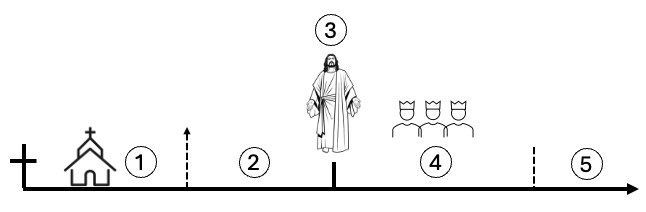
\includegraphics[width=\textwidth]{images/premillennialism.png}
    \caption{前千禧年觀}
    \label{fig:premillennialism}
\end{figure}

\section*{後千禧年}
後千禧年的解釋，是\ding{172}教會時期，然後是\ding{173}千禧年，然後\ding{174}耶穌再度降臨，最後是\ding{175}新天新地。 

\begin{figure}[htbp]
    \centering
    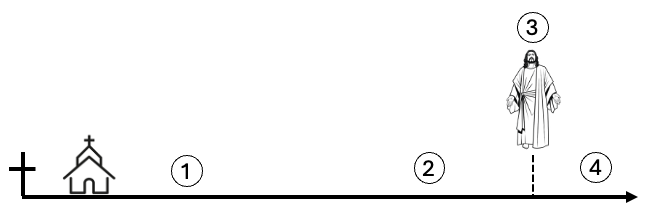
\includegraphics[width=\textwidth]{images/postmillennialism.png}
    \caption{後千禧年觀}
    \label{fig:postmillennialism}
\end{figure}

\section*{無千禧年}
無千禧年的解釋，是現在的\ding{172}教會時期就是千禧年，然後\ding{173}耶穌再度降臨，然後\ding{174}新天新地。 

\begin{figure}[htbp]
    \centering
    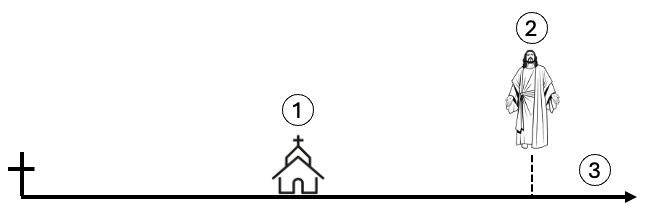
\includegraphics[width=\textwidth]{images/amillennialism.png}
    \caption{無千禧年觀}
    \label{fig:amillennialism}
\end{figure}


\begin{table}[htbp]
\centering
\small
\renewcommand{\arraystretch}{1.1}
\renewcommand{\thetable}{附錄\arabic{chapter}.\arabic{table}}% local to this table
\begin{minipage}{\linewidth}
\centering
\caption{三種千禧年觀的比較}\label{tab:millennium}
\begin{tabular}{p{0.12\linewidth}p{0.25\linewidth}p{0.25\linewidth}p{0.25\linewidth}}
\hline
列表 & 前千禧年觀 & 後千禧年觀 & 無千禧年觀 \\
\hline
英文 &
{\footnotesize Pre\-millennialism}\footnote{前千禧年論的代表人物：殉道者游斯丁（Justin Martyr）、愛任紐（Irenaeus）、特土良（Tertullian）、華富爾（John F. Walvoord）、萊里（Charles Ryrie）。} &
{\footnotesize Post\-millennialism}\footnote{後千禧年論的代表人物：愛德華滋（Jonathan Edwards）、賀智（Charles Hodge）、史普羅（R. C. Sproul）。} &
{\footnotesize A\-millennialism}\footnote{無千禧年論的代表人物：奧古斯丁（Augustine）、加爾文（John Calvin）、比爾（G. K. Beale）。} \\
基督再來 & 在千禧年之前 & 在千禧年之後 & 在千禧年（教會時代）之後 \\
千禧年 & 基督再來之後在地上實際統治1,000年 & 福音在世上大有能力的時期，帶來廣泛的歸信、公義與和平；通常理解為象徵性，而非字面上的一千年 & 教會時代，象徵性的「一千年」，即基督現今在天上的統治 \\
撒但被捆綁 & 千年完了暫時被釋放，然後被扔在火湖裡 & 大受限制，不能攔阻福音傳到萬國；捆綁發生在千禧年之前或期間 & 不能攔阻福音傳給萬國；但他並非毫無作為，仍繼續敵擋神的子民 \\
復活 & 兩個階段：信徒在千禧年之前或開始時復活；不信者在千禧年之後復活受審判 & 基督再來時，信與不信的人一次普遍復活 & 同後千禧年論 \\
最後叛亂 & 千禧年之後 & 千禧年將結束時 & 現今世代結束時 \\
\hline
\end{tabular}
\end{minipage}
\end{table}
